\subsubsection{BLDC-Motor}
Der Antrieb für den Ballabwurf ist realisiert mittels eines
Brushless-Gleichstrommotors vom Modell A20-12XL EVO von Hacker.
Dieser wird mittels eines passenden kommerziellen Reglers vom
Typ X-30 PRO betrieben. Der Regler wird gestellt durch die Firmware
des Freedomboards, welche per UART bedient wird.

Die zugehörige Software kann mittels des UART-Interfaces per
Kommandozeile bedient werden mit dem Befehl \verb!BLDC! und den
zugehörigen Parametern. Die komplette Liste aller Befehle zu
\verb!BLDC! kann mittels \verb!BLDC help! aufgerufen werden.

\begin{figure}[h!]
	\centering
	\begin{subfigure}[b]{0.45\textwidth}
		\centering
		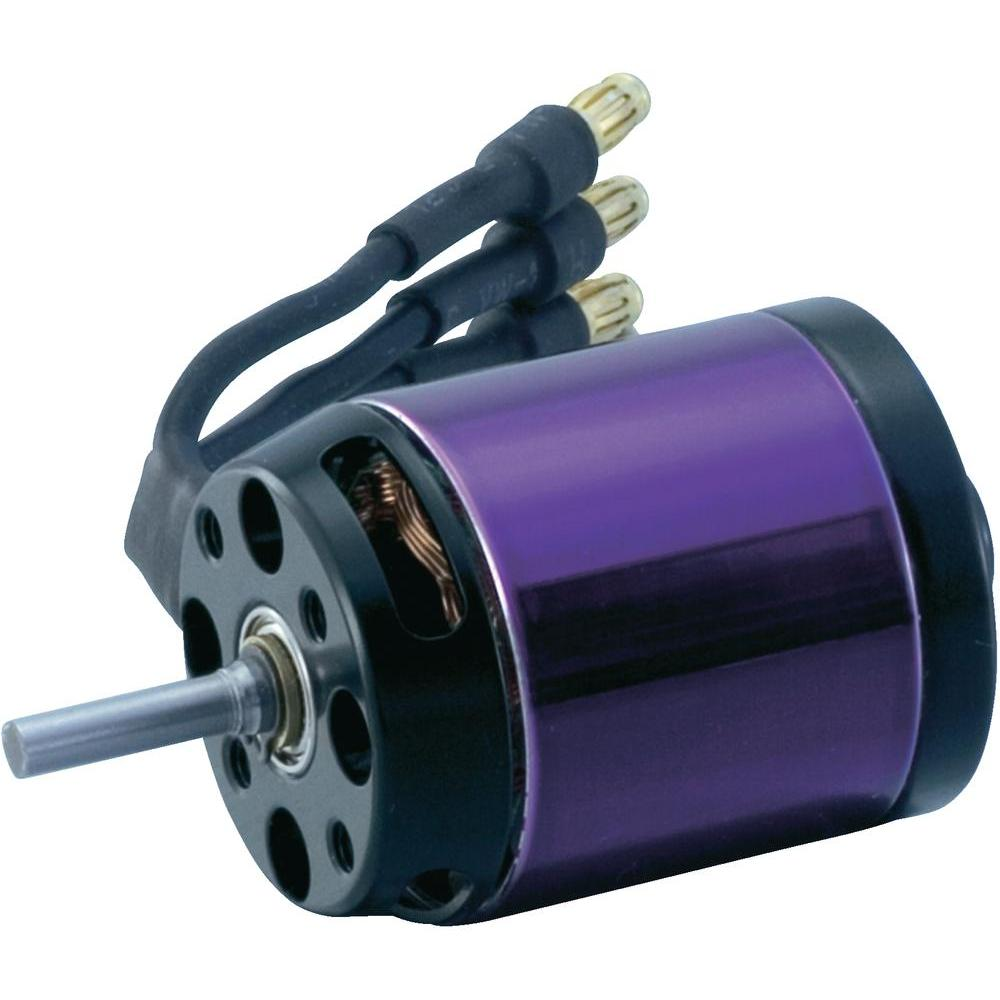
\includegraphics[width=0.75\textwidth]{../../fig/et/a20_12xl_evo.jpg}
		\caption{BLDC-Motor Hacker A20-12XL EVO}
	\end{subfigure}
	\begin{subfigure}[b]{0.45\textwidth}
		\centering
		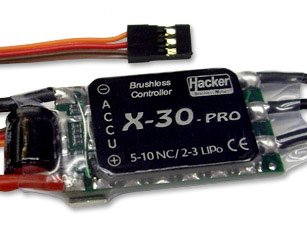
\includegraphics[width=0.75\textwidth]{../../fig/et/x30_pro.jpg}
		\caption{BLDC-Motor Hacker X-30 PRO}
	\end{subfigure}
	\caption{Antriebssystem für den Ballabwurf}
\end{figure}

Da ein kommerzieller Regler aus dem Modellbau verwendet wird, 
kann lediglich ein Standard PWM-Signal aus dem Modellbau benutzt werden, 
um die Drehzahl des Motors zu stellen. Da dieser Regler eine echte 
Drehzahlregelung implementiert wird auf einen überlagerten Regler 
auf dem Freedomboard verzichtet.
Eine allfällige Parametrierung kann mittels eines Programmieradapters
X-PRO USB Controller V2 des Herstellers vorgenommen werden.
